% ---------------------------------------------------------------------------
% Continual Learning as Schrodinger Bridge Transport Between Posteriors
% ICASSP format: 4 pages of content + 1 page of references only.
%
% Build:  tectonic icassp.tex        (or pdflatex + bibtex + pdflatex x2)
% Needs:  spconf.sty, IEEEbib.bst, refs.bib, figures/ -- all in this folder.
%
% Before submitting, check the current call for the anonymity policy; if
% review is double-blind, replace \name and \address with "Anonymous".
% ---------------------------------------------------------------------------
\documentclass{article}
\usepackage{spconf,amsmath,amssymb,graphicx,booktabs}
\usepackage[T1]{fontenc}
\usepackage{algorithm}
\usepackage[noend]{algpseudocode}
\usepackage{microtype}
\usepackage[hidelinks]{hyperref}
\usepackage{xcolor}
% Claims awaiting measurements; must all be gone before submission.
\newcommand{\tbd}[1]{\textcolor{red}{#1}}

\newcommand{\Dt}{\mathcal{D}}
\newcommand{\Lh}{\mathcal{L}}
\newcommand{\KL}{\mathrm{KL}}
\newcommand{\Rb}{\mathbb{R}}
\newcommand{\Eb}{\mathbb{E}}
\newcommand{\Nc}{\mathcal{N}}
\newcommand{\thk}{\theta_t^{(k)}}
\makeatletter
\newcommand{\mastheadcaption}{\def\@captype{figure}\caption}
\makeatother

\title{Continual Learning as Schr\"odinger Bridge Transport Between Posteriors}
\name{Anand Ravishankar}
\address{Stony Brook University, Stony Brook, NY, USA}

\begin{document}
\ninept

% Masthead under the title block.
\twocolumn[{%
  \renewcommand\twocolumn[1][]{#1}%
  \maketitle
  \vspace{-1.2em}
  \begin{center}
    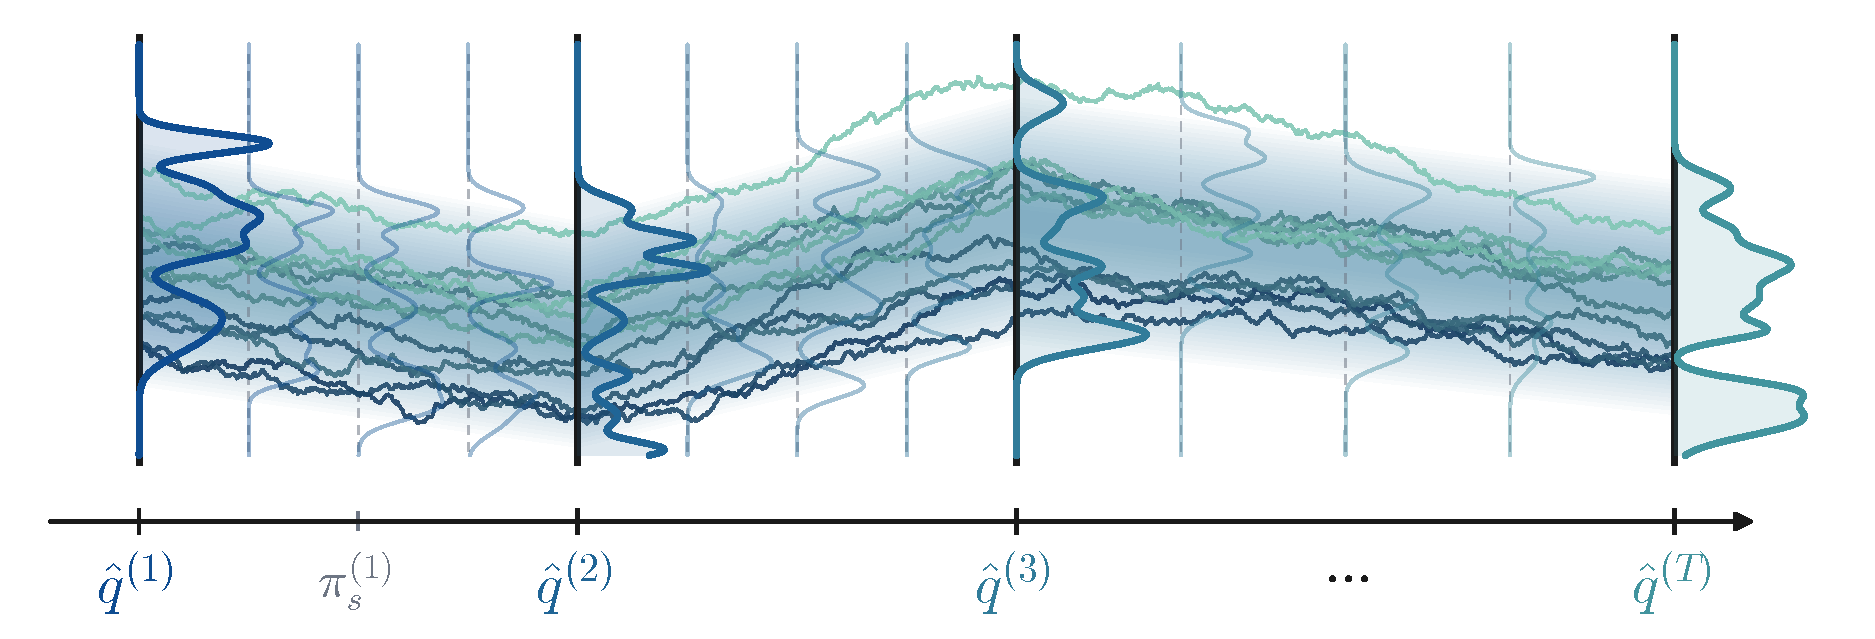
\includegraphics[width=\textwidth]{figures/fig_masthead.pdf}
    \vspace{-1.6em}
    \mastheadcaption{Continual learning as a chain of $T-1$ Schr\"odinger bridges
    between sequential posteriors $q_t = p(\theta\mid\Dt_{1:t})$. Bold
    verticals are task boundaries, dashed verticals are intermediate marginals
    $\pi_\beta$ of one bridge, and the shaded tube is the marginal envelope.
    Each path is one network of the population, coloured by where it started:
    the same networks are transported across every boundary rather than
    re-fitted, and the bridge determines which start is carried to which end.
    Densities are schematic.}
    \label{fig:masthead}
  \end{center}
  \vspace{0.6em}
}]

\begin{abstract}
Continual learning without replay is usually posed as constrained
optimisation: fit the incoming task while a penalty holds the weights near an
earlier solution. We pose each task boundary instead as a transport problem
between consecutive posteriors. Sequential Bayes fixes both endpoints but not
the path. We show that the geometric path between them has a score that splits
exactly into a tempered likelihood gradient and a Fisher-weighted prior force,
and that annealed Langevin dynamics along it, the natural reference process,
lags the path at any finite speed. The minimal correction is a Schr\"odinger
bridge. We transport a population of networks across each boundary and learn
the bridge drift by iterative Markovian fitting over per-neuron weight tokens,
so that one drift, conditioned on the local likelihood and prior forces, is
amortised across the task stream. With one shared head and no stored examples
the method reaches $91.0\%$ average accuracy on $10$-task Permuted MNIST,
against $84\%$, $86\%$ and $90\%$ reported for EWC, SI and VCL with the same
network, and the learned drift carries later boundaries at a quarter of the
reference cost for a $0.2$-point loss.
\end{abstract}

\begin{keywords}
Continual learning, Schr\"odinger bridge, sequential Bayesian inference,
optimal transport, catastrophic forgetting
\end{keywords}

% ===========================================================================
\section{Introduction}
\label{sec:intro}

% STYLE: modelled on recent ICASSP continual-learning papers (Vander Eeckt &
% Van hamme, ICASSP 2023/2026): application first, taxonomy, enumerated
% limitations, "In this paper, we propose", inline threefold contributions.
%
% \tbd{...} (red) marks claims NOT yet supported by measurements. Current TPU
% sweep (20 seeds, 10-task Permuted MNIST, K=128): PSB 0.912; EWC K=128 0.946;
% SI K=128 0.930; beta=1 variant 0.922; single-network EWC 0.901, SI 0.878.
% PSB currently beats only single-network EWC/SI and published VCL.
% Replace every \tbd{} with measured results before submission.

Automatic speech recognition (ASR) and other audio models are increasingly
deployed in settings that keep changing after training: a recogniser must adapt
to new speakers, accents, domains and recording
conditions~\cite{vandereeckt2023weight,vandereeckt2026inverse}. Yet such
adaptation causes catastrophic
forgetting~\cite{goodfellow2013empirical,kirkpatrick2017ewc}, where performance
on previously learned conditions degrades. Retraining on all past data avoids
this but is often impossible, since recordings may not be stored for privacy or
storage reasons. Continual learning (CL) addresses this setting by learning a
sequence of tasks without revisiting earlier data, balancing plasticity on the
new task against stability on the old
ones~\cite{wang2024survey,mirzadeh2020regimes}.

CL methods are commonly grouped into three
families~\cite{wang2024survey,vandeven2022types}. Architectural methods add
task-specific capacity~\cite{vandereeckt2023adapters}, and rehearsal methods
replay a stored memory of past samples, which privacy constraints may forbid.
Regularisation-based methods are memory-free and keep a single shared model:
EWC~\cite{kirkpatrick2017ewc}, its online variant~\cite{schwarz2018progress} and
SI~\cite{zenke2017si} penalise changes to parameters that were important for
earlier tasks, while Bayesian methods such as VCL~\cite{nguyen2018vcl} carry an
approximate posterior forward as the next prior. These methods share two
limitations: (1) they summarise all earlier tasks by a single Gaussian around a
single solution, although the posterior over network weights is strongly
multimodal, so approximation errors compound from task to
task~\cite{kessler2023sequential,melo2025tdvcl} and the importance estimates
themselves can be unreliable~\cite{liu2026ewcdr}; (2) the penalty specifies
where the model should end up but not how to get there, leaving the transition
between tasks to the optimiser, whose training regime alone changes forgetting
substantially~\cite{mirzadeh2020regimes}.

In this paper, we propose \emph{Posterior Schr\"odinger Bridges} (PSB), which
treats each task boundary as transport between consecutive posteriors.
Sequential Bayes fixes both endpoints, $p(\theta\mid\Dt_{1:t})$ and
$p(\theta\mid\Dt_{1:t+1})$, but not the path between them. Rather than
penalising departures from one old solution, PSB moves a population of networks,
which captures several modes as deep ensembles
do~\cite{lakshminarayanan2017ensembles,wilson2020bayesian}, along the geometric
path from the old posterior to the new one. The score of this path splits
exactly into a tempered likelihood gradient and a Fisher-weighted prior force,
so EWC-type penalties are recovered as a special case. The least-effort
transport between two given distributions is a Schr\"odinger bridge
(SB)~\cite{leonard2014survey}, the same data-to-data formulation that has
recently advanced generative speech
enhancement~\cite{jukic2024sb,richter2025objectives}; we learn its drift over
per-neuron weight tokens and amortise it across task boundaries.

Our contributions are threefold: (i)~we formulate replay-free CL as
Schr\"odinger-bridge transport between sequential posteriors and show that its
reference score unifies the likelihood and Fisher-prior forces used by
regularisation-based methods; (ii)~we propose PSB, which learns the bridge
drift by iterative Markovian fitting over per-neuron weight tokens and keeps a
state that does not grow with the number of tasks; (iii)~on Permuted, Rotated
and Split MNIST with a single shared head and no stored examples, \tbd{PSB
consistently outperforms EWC, online EWC, SI and VCL, including ensembles of
the same size}, while ablations confirm the effect of each component.

% ===========================================================================
\section{Background}
\label{sec:background}

\textbf{Sequential Bayes.} Let $\theta\in\Rb^P$ collect the weights of one
network shared by all tasks and let $q_t(\theta)=p(\theta\mid\Dt_{1:t})$. If the
datasets are conditionally independent given $\theta$,
\begin{equation}
q_{t+1}(\theta) \;\propto\; \Lh_{t+1}(\theta)\,q_t(\theta),
\qquad \Lh_{t+1}(\theta)=p(\Dt_{t+1}\mid\theta).
\label{eq:seqbayes}
\end{equation}
Thus $q_t$ is a sufficient summary of the past. The obstacle is
representational: written out, $q_t\propto p(\theta)\prod_{i\le t}\Lh_i(\theta)$
needs every past dataset to evaluate, so a replay-free learner must replace it
with a lossy summary, and because \eqref{eq:seqbayes} is recursive each
boundary's approximation error becomes the next boundary's prior
error~\cite{kessler2023sequential}.

\textbf{Schr\"odinger bridges.} Given a reference path measure $Q$ on $[0,1]$ and
marginals $\pi_0,\pi_1$, the SB problem~\cite{leonard2014survey} is
\begin{equation}
P^\star=\operatorname*{arg\,min}_{P}\ \KL(P\,\|\,Q)
\quad\text{s.t.}\quad P_0=\pi_0,\;P_1=\pi_1 .
\label{eq:sb}
\end{equation}
If $Q$ is a diffusion $d\theta_s=b(\theta_s,s)\,ds+\sigma\,dW_s$ and $P$ has
drift $b+u$, Girsanov's theorem gives
$\KL(P\|Q)=\tfrac{1}{2\sigma^2}\Eb_P\!\int_0^1\|u_s\|^2 ds$: $P^\star$ reaches
$\pi_1$ with the least control effort added to the reference, and as
$\sigma\to0$ it becomes an optimal transport problem whose cost is that
effort~\cite{leonard2014survey}. $P^\star$ is the unique measure that
is Markov and lies in the \emph{reciprocal class} of $Q$, the mixtures of $Q$'s
bridges over some endpoint coupling. IMF~\cite{shi2023dsbm,peluchetti2023idbm}
finds it by alternating a Markovian projection, which regresses a drift onto
paths of the current coupling, with a reciprocal projection, which regenerates
the coupling by simulating the fitted process.

% ===========================================================================
\section{Posterior Schr\"odinger Bridges}
\label{sec:method}

\subsection{The posterior bridge}
\label{sec:bridge}

\textbf{Representation.} We carry $K$ networks $\{\thk\}_{k=1}^K$ and a
diagonal precision $\Lambda_t\in\Rb^P_{+}$, and approximate
\begin{equation}
q_t(\theta)\;\approx\;\tfrac1K\textstyle\sum_{k}\Nc\big(\theta;\,\thk,\,(\lambda\Lambda_t)^{-1}\big),
\label{eq:mixture}
\end{equation}
with $\lambda$ a prior-strength constant. The particles carry multimodal
structure; the shared precision gives every component support in all $P$
directions. After task $t$, $\Lambda_t=\gamma\Lambda_{t-1}+F_t$, where $F_t$ is
the diagonal Fisher of task $t$ averaged over particles and scaled to unit mean,
and $\gamma<1$ discounts older curvature so the prior does not stiffen uniformly
over a long stream. $F_t$ is exact per example: a linear layer's per-example
gradient is an outer product $\delta_n a_n^{\top}$, so
$\sum_n(\delta_n a_n^{\top})^{\odot2}=(\delta^{\odot2})^{\top}a^{\odot2}$ is
one matrix product per layer.

\textbf{The path.} Across the boundary $t\to t+1$ define, for
$\beta\in[0,1]$,
\begin{equation}
\pi_\beta(\theta)\;\propto\;\Lh_{t+1}(\theta)^{\beta}\,q_t(\theta)
\;=\;q_t(\theta)^{1-\beta}\,q_{t+1}(\theta)^{\beta},
\label{eq:path}
\end{equation}
where the equality uses \eqref{eq:seqbayes}. This is the geometric path of
annealed importance sampling and SMC
samplers~\cite{neal2001ais,delmoral2006smc}, and it runs exactly from $q_t$ to
$q_{t+1}$. It tempers the \emph{likelihood} rather than corrupting the
\emph{parameters}, so every $\pi_\beta$ is a posterior over functioning
networks. This matters in weight space: with $K\le256$ samples in
$P=89{,}610$ dimensions, isotropic forward noise puts over $99.99\%$ of its
energy outside the span of the samples, where no score can be estimated, so a
data-to-noise construction cannot be inverted.

We transport each mixture component separately. Reweighting components by
their evidence under $\Lh_{t+1}^{\beta}$ would be exact, but with
$60{,}000$ examples the weights are degenerate: the effective sample size of
$32$ particles collapses to $1.4$. For particle $k$ the score of the path is
\begin{equation}
\nabla_\theta\log\pi^{(k)}_\beta(\theta)
=\underbrace{-\beta\,\nabla_\theta\ell_{t+1}(\theta)}_{\text{tempered likelihood}}
\;\underbrace{-\;\lambda\Lambda_t\big(\theta-\thk\big)}_{\text{Fisher-weighted prior}},
\label{eq:score}
\end{equation}
with $\ell_{t+1}$ the mean negative log-likelihood of task $t{+}1$. The second
term is the gradient of the EWC penalty, but here it is balanced against a
likelihood whose weight grows with $\beta$. Setting \eqref{eq:score} to zero,
\begin{equation}
\theta-\thk\;=\;-\tfrac{\beta}{\lambda}\,\Lambda_t^{-1}\,\nabla_\theta\ell_{t+1}(\theta),
\label{eq:equilibrium}
\end{equation}
so displacement grows with $\beta$ and is rationed per coordinate by
$1/\Lambda_{t,j}$: weights that earlier tasks rely on barely move, weights they
left free absorb the new task. Since \eqref{eq:equilibrium} is nonlinear with
many roots, sweeping $\beta$ upward from $0$ is a numerical continuation: it
follows the solution branch that starts at the old network instead of jumping
to an arbitrary minimiser of the new task.

\subsection{Reference process and the bridge problem}
\label{sec:reference}

The SB cost is measured against a reference. Brownian motion, the usual choice,
is a poor one here: its cost is Euclidean length, which prices a small move in a
critical weight like a large move in an irrelevant one, and its bridges are
straight lines through regions where interpolated networks fail. We instead take
as reference $Q$ the annealed Langevin diffusion along the path,
\begin{equation}
d\theta_s=\nabla_\theta\log\pi^{(k)}_{\beta(s)}(\theta_s)\,ds+\sqrt{2\tau}\,dW_s,
\quad \beta(s)\colon 0\nearrow1 .
\label{eq:reference}
\end{equation}
Its drift is \eqref{eq:score}, so moving a weight against its prior costs
control effort in proportion to $\Lambda_{t,j}$: the Fisher metric enters through
the reference instead of being imposed.

At temperature $\tau=1$ and run infinitely slowly, \eqref{eq:reference} keeps
$\pi_{\beta(s)}$ as its marginal at every $s$ and ends at $q_{t+1}$. At finite speed it \emph{lags}: the
population is still relaxing toward $\pi_{\beta(s)}$ when $\beta$ has moved on,
and it ends short of $q_{t+1}$. The posterior bridge
\begin{equation}
P^\star_t=\operatorname*{arg\,min}_{P}\ \KL(P\,\|\,Q)
\quad\text{s.t.}\quad P_0=q_t,\;P_1=q_{t+1}
\label{eq:psb}
\end{equation}
is the smallest correction to \eqref{eq:reference} that removes the lag. By
Doob's $h$-transform its drift is the reference drift plus a correction, so the
learned drift need not be exact: we deploy it alongside a few reference moves
that correct its residual error.

\textbf{Discretisation.} Each boundary is split into $M$ stages with
$\beta_m=m/M$, and each stage applies $n$ moves of the $\tau\to0$ limit of
\eqref{eq:reference}, split into its two terms:
\begin{equation}
\theta\leftarrow\theta-\beta_m\,\eta\,\mathcal{P}(g),\qquad
\theta\leftarrow\frac{\theta+w\odot\thk}{1+w},\quad w=\lambda\eta\Lambda_t ,
\label{eq:moves}
\end{equation}
where $g$ is a minibatch gradient of $\ell_{t+1}$, $\mathcal{P}$ the Adam
preconditioner, and division is elementwise. The second step is the exact
proximal operator of the prior term. Adding the prior to the loss instead would
route its gradient through $\mathcal{P}$, which divides each coordinate by its
own gradient scale and cancels exactly the $\Lambda$-weighting the prior exists
to impose; applied proximally the weighting survives and the step is stable for
any $w$. At $\tau\to0$ particles track the path rather than sample it, and the
population supplies the spread.

\textbf{Special cases.} With $M=1$ the path collapses to $\beta=1$ and
\eqref{eq:moves} is EWC with a decayed Fisher, applied proximally and run on
$K$ networks; with $K=1$ as well it is a single EWC-style learner. PSB therefore
differs from this family only in transporting along $\pi_\beta$, and
Fig.~\ref{fig:path} isolates exactly that difference.

\subsection{Learning the bridge by IMF over neuron tokens}
\label{sec:imf}

\textbf{Tokens.} Regression over $\theta\in\Rb^{89{,}610}$ from $K=128$ networks
has $1.4\times10^{-3}$ samples per dimension. A network is also a set of
neurons: a layer with $n_\ell$ units and fan-in $d_\ell$ yields $n_\ell$ tokens
$z\in\Rb^{d_\ell+1}$ (incoming weights and bias). The map is invertible, and
tokens of a layer share one regression, giving $16$, $127$ and $13$ samples per
dimension for our three layers from a single snapshot of the population.

\textbf{Drift.} Per layer we fit $d_\phi(z,g,a,\beta)$, the displacement
$\Delta z$ of a token over one stage given its value $z$, its likelihood-gradient
token $g$, its prior-force token $a$ (the two terms of \eqref{eq:score}), and
$\beta$:
\begin{equation}
\min_\phi\ \Eb\,\big\|\,d_\phi(z,g,a,\beta)-\Delta z\,\big\|^2 .
\label{eq:markov}
\end{equation}
This is IMF's Markovian projection. Conditioning on forces rather than on task
identity makes $d_\phi$ a rule, how far to move under this much evidence against
this much stiffness, so a drift fitted on early boundaries applies to later
ones. $d_\phi$ is an MLP on RMS-normalised inputs, their log-scales and Fourier
features of $\beta$, with a zero-initialised output layer so that an unfitted
drift leaves the reference unchanged.

\textbf{IMF along the stream.} The first $W$ boundaries use the reference
($n=n_{\mathrm{ref}}$) and record per-stage displacements. Each IMF round then
fits a forward half-bridge $d_\phi$ by \eqref{eq:markov} and a backward
half-bridge $d_\psi$ on reversed pairs $(z{+}\Delta z\mapsto-\Delta z)$, and
discards the recorded coupling. The next boundary is traversed with the drift,
one drift step per stage followed by $n_{\mathrm{dep}}\ll n_{\mathrm{ref}}$
reference moves, and its displacements become the new coupling: this
re-simulation is the reciprocal projection. At the bridge the half-bridges
invert each other, so the cycle residual
\begin{equation}
\mathcal{C}=\Eb\big\|d_\phi(z)+d_\psi\big(z+d_\phi(z)\big)\big\|^2\big/\,\Eb\|d_\phi(z)\|^2
\label{eq:cycle}
\end{equation}
measures the distance from the fixed point. The task stream thus supplies IMF's
iterations; after $R$ rounds the drift is frozen (Algorithm~\ref{alg:psb}).

\begin{algorithm}[t]
\caption{Posterior Schr\"odinger Bridges (PSB)}
\label{alg:psb}
\small
\begin{algorithmic}[1]
\Require tasks $\Dt_{1:T}$; $K$, $M$, $n_{\mathrm{ref}}$, $n_{\mathrm{dep}}$, $W$, $R$, $\lambda$, $\gamma$
\State Train $K$ networks on $\Dt_1$ independently; $\Lambda_1\gets F_1$
\For{$t=1,\ldots,T-1$}
  \State Freeze centres $\thk$; $n\gets n_{\mathrm{dep}}$ if $d_\phi$ fitted, else $n_{\mathrm{ref}}$
  \For{$m=1,\ldots,M$} \Comment{$\beta_m=m/M$}
    \State \textbf{if} $d_\phi$ fitted: move every token by $d_\phi(z,g,a,\beta_m)$
    \State Apply $n$ moves \eqref{eq:moves}; record $(z,g,a,\beta_m,\Delta z)$
  \EndFor
  \If{$W\le t<W+R$} \Comment{one IMF round}
    \State Fit $d_\phi$, $d_\psi$ by \eqref{eq:markov}; clear the record
  \EndIf
  \State $\Lambda_{t+1}\gets\gamma\Lambda_t+F_{t+1}$
\EndFor
\State \Return ensemble $\tfrac1K\sum_k p(y\mid x,\thk)$
\end{algorithmic}
\end{algorithm}

% ===========================================================================
\section{Experiments}
\label{sec:experiments}

\textbf{Setup.} \emph{Permuted MNIST}~\cite{goodfellow2013empirical}: $10$
tasks, each a fixed pixel permutation, the first being the identity.
\emph{Rotated MNIST}: $10$ tasks rotated by $0^\circ,20^\circ,\ldots,180^\circ$.
\emph{Split MNIST}~\cite{zenke2017si}: $5$ tasks on digit pairs, evaluated
domain-incremental (a shared binary head) and class-incremental (a shared
$10$-way head)~\cite{vandeven2019three}. The network is a $784$--$100$--$100$
ReLU MLP with one shared head and no task-specific parameters ($P=89{,}610$ for
Permuted MNIST), the network behind the published Permuted MNIST results for
EWC, SI, LP and VCL~\cite{nguyen2018vcl}. We use $K=128$; Adam with
$\eta=10^{-3}$ and batch $64$; $3{,}000$ steps on task $1$; $M=25$ stages with
$n_{\mathrm{ref}}=100$; $\lambda=4$, $\gamma=0.8$; and Fisher from $20{,}000$
examples. The drift has two hidden layers of width $512$, is trained for
$3{,}000$ AdamW steps on tokens from $8$ particles, and is deployed with step
scale $0.3$, $W=R=3$ and $n_{\mathrm{dep}}=25$. With $a_{i,j}$ the accuracy on
task $j$ after task $i$, we report average accuracy
$\tfrac1T\sum_j a_{T,j}$, forgetting
$\tfrac1{T-1}\sum_{j<T}\big(\max_{j\le i<T}a_{i,j}-a_{T,j}\big)$, and
acquisition $\tfrac1T\sum_j a_{j,j}$, which separates failing to learn from
failing to retain. Results are means over five seeds; rows marked $\dagger$ are
single runs.

\begin{table}[t]
\centering
\caption{Ten-task Permuted MNIST, single head, no stored examples. Published
results use the same $784$--$100$--$100$--$10$ network~\cite{nguyen2018vcl};
coreset variants of VCL store examples and are excluded.}
\label{tab:main}
\setlength{\tabcolsep}{5pt}
\begin{tabular}{lccc}
\toprule
Method & Avg.\ acc. & Forgetting & Acquisition \\
\midrule
LP~\cite{nguyen2018vcl} & $0.82$ & -- & -- \\
EWC~\cite{kirkpatrick2017ewc} & $0.84$ & -- & -- \\
SI~\cite{zenke2017si} & $0.86$ & -- & -- \\
VCL~\cite{nguyen2018vcl} & $0.90$ & -- & -- \\
\midrule
PSB & $0.910\pm0.001$ & $0.035$ & $0.941$ \\
PSB, $4{,}000$ moves$^\dagger$ & $\mathbf{0.914}$ & $\mathbf{0.034}$ & $\mathbf{0.945}$ \\
\bottomrule
\end{tabular}
\end{table}

\textbf{Comparison.} Table~\ref{tab:main} compares PSB with published
results for the same network. PSB reaches $0.910$ with seed spread $0.001$,
above VCL's $0.90$, and a longer traversal of $4{,}000$ moves per boundary
reaches $0.914$. Forgetting is low and uniform: seed-averaged accuracies on
tasks $1$--$10$ after the full stream are $0.937$, $0.913$, $0.913$, $0.913$,
$0.872$, $0.899$, $0.905$, $0.916$, $0.908$ and $0.922$, with the oldest task
the most accurate.

\begin{figure}[t]
\centering
\includegraphics[width=0.94\columnwidth]{figures/fig2_path.pdf}
\vspace{-0.6em}
\caption{The path, not the budget. Moves \eqref{eq:moves} with $\beta$ swept
$0\to1$ (blue) versus the same moves with $\beta$ fixed at $1$ (red), as the
number of moves per boundary grows; $K=32$, all else matched.}
\label{fig:path}
\end{figure}

\textbf{The path, not the budget.} Because $\beta$ scales the data step, the
bridge could be mistaken for a learning-rate warm-up. Fig.~\ref{fig:path}
separates the two. As the budget grows from $2{,}500$ to $20{,}000$ moves per
boundary, traversal along $\pi_\beta$ improves from $0.901$ to $0.912$, while
the same moves with $\beta$ fixed at $1$ \emph{degrade} from $0.889$ to
$0.879$. Off the path, extra moves raise acquisition ($0.954\to0.958$) but raise
forgetting faster ($0.073\to0.088$), buying the new task at the old tasks'
expense; on the path, acquisition rises ($0.949\to0.956$) while forgetting
falls ($0.053\to0.049$). Under identical budgets the curves move in opposite
directions, so the gain comes from the path. That the blue curve has not
saturated at $20{,}000$ moves is the finite-time lag of
Sec.~\ref{sec:reference}, the quantity the bridge exists to remove.

\begin{table}[t]
\centering
\caption{Learning the bridge ($K=128$). Top: IMF rounds; explained variance of
the forward and backward half-bridges and cycle residual \eqref{eq:cycle}.
Bottom: kernel moves per boundary once the drift is deployed.}
\label{tab:bridge}
\setlength{\tabcolsep}{4.5pt}
\begin{tabular}{lccc}
\toprule
IMF round & fwd.\ $R^2$ & bwd.\ $R^2$ & cycle $\mathcal{C}$ \\
\midrule
1 (bridge matching) & $0.286$ & $0.168$ & $0.908$ \\
2 & $\mathbf{0.624}$ & $\mathbf{0.666}$ & $\mathbf{0.114}$ \\
\midrule
Traversal & moves & Avg.\ acc. & Forgetting \\
\midrule
Reference & $2{,}500$ & $0.910$ & $0.035$ \\
Drift$^\dagger$ & $2{,}500$ & $0.910$ & $0.035$ \\
Drift$^\dagger$ & $\phantom{0}\mathbf{625}$ & $0.908$ & $0.028$ \\
\bottomrule
\end{tabular}
\end{table}

\textbf{Learning the bridge.} Table~\ref{tab:bridge} (top) shows IMF
converging. After one round, which is bridge matching, the half-bridges explain
$29\%$ and $17\%$ of the stage displacement and do not invert each other
($\mathcal{C}=0.908$). After a second round, fitted on the coupling that the
first drift generated, they explain $62\%$ and $67\%$ and nearly invert
($\mathcal{C}=0.114$). Closing the cycle does not raise final accuracy: at
$K=32$, $\mathcal{C}$ falls from $0.274$ to $0.104$ while accuracy moves from
$0.9015$ to $0.9017$, and at $K=128$ it moves from $0.907$ to $0.904$. The
endpoints of each bridge are fixed by \eqref{eq:path}; the bridge governs how
cheaply they are connected, not where they lie. This matches the view of
Kessler et al.~\cite{kessler2023sequential} that continual learning under
sequential Bayes is limited by how well each posterior is represented. The
bottom of Table~\ref{tab:bridge} measures that cost. At the reference budget the
drift matches the reference ($0.9103$ vs.\ $0.9099$); with a quarter of the
moves it reaches $0.908$. Since the first $W=3$ boundaries use the reference,
total moves over this $10$-task stream halve, and the saving approaches $4\times$
as the stream grows.

\begin{table}[t]
\centering
\caption{Average accuracy against prior strength $\lambda$, five seeds
(s.d.\ $\le0.009$). Forgetting at $\lambda=16$ is $0.37$ and $0.41$.}
\label{tab:other}
\setlength{\tabcolsep}{4.5pt}
\begin{tabular}{lccccc}
\toprule
$\lambda$ & $1$ & $2$ & $4$ & $8$ & $16$ \\
\midrule
Rotated & -- & $0.540$ & $0.551$ & $0.568$ & $\mathbf{0.593}$ \\
Split, domain & $0.636$ & -- & $0.649$ & -- & $\mathbf{0.662}$ \\
\bottomrule
\end{tabular}
\end{table}

\textbf{Other benchmarks.} Table~\ref{tab:other} reports Rotated and
domain-incremental Split MNIST. Accuracy rises monotonically with $\lambda$ on
both and has not peaked at $\lambda=16$, so the best setting lies at or beyond
the values tested. Both are markedly harder for PSB than Permuted MNIST, with
forgetting ten times higher. We attribute this to the diagonal precision:
different permutations load largely different input weights, which a diagonal
$\Lambda$ can protect separately, whereas rotations and digit pairs reuse the
same pixels with conflicting targets, which a coordinate-wise prior cannot
arbitrate. Structured precisions~\cite{ritter2018laplace} are the natural
extension and slot into \eqref{eq:score} unchanged. Class-incremental Split
MNIST reaches $0.224\pm0.009$ against a chance level of $0.20$: with two
classes per task nothing trains the absent classes' logits, an output-layer
failure that no weight-space prior addresses and that we leave out of scope.

\textbf{Limitations.} Baselines are quoted from~\cite{nguyen2018vcl} for the
same network; training schedules and tuning may differ, and we have not re-run
them. PSB predicts with a $K$-member ensemble, and ensembling alone improves
accuracy~\cite{lakshminarayanan2017ensembles}. The $\beta{=}1$ curve of
Fig.~\ref{fig:path} is an ensemble of the same size with the same prior and
trails PSB at every budget, but it is a $K=32$ proximal variant; a standard EWC
ensemble at $K=128$ remains the cleaner control. Persistent state is $K$
networks, $\Lambda_t$ and a $2.9$M-parameter drift, independent of $T$ but
larger than VCL's $2P$. We work at $\tau\to0$, so particles track rather than
sample each $\pi_\beta$.

% ===========================================================================
\section{Conclusion}
\label{sec:conclusion}

Posing the continual-learning task boundary as transport between consecutive
posteriors identifies the geometric path as the route and the Schr\"odinger
bridge as the way to traverse it in finite time. Tempering the likelihood rather
than corrupting the weights keeps every intermediate distribution a posterior
over working networks, which is what makes a bridge viable in weight space, and
the score of that path recovers the likelihood and Fisher-prior forces that
replay-free methods use, now tied together by a schedule with a precise meaning.
A drift learned by iterative Markovian fitting over neuron tokens converges
toward the bridge and carries later boundaries at a fraction of the cost.
Structured precisions and bridges between function-space posteriors are the
natural next steps.

\vfill\pagebreak
\bibliographystyle{IEEEbib}
\bibliography{refs}

\end{document}
